\section{Fortran--PyTorch equivalence verification}
\label{sec:fortran-torch-equivalence}

The verification distinguishes the translated SURF process sequence from the
standalone reconstruction of the atmospheric surface-layer boundary. In a
coupled OpenIFS forecast, the surface roughness lengths and the
surface-layer turbulent exchange coefficients are supplied by the
atmospheric physics. In an offline integration they must instead be
diagnosed from the meteorological forcing. The first experiment therefore
holds all Fortran roughness, surface-layer exchange, and radiation boundary
arrays fixed when integrating the SURF update with PyTorch under those boundaries. The second
experiment lets the Fortran and PyTorch implementations construct their own
roughness and surface-layer exchange states from the same forcing. This
separation tests the numerical translation and the standalone interface
without conflating the two questions.

All regional experiments use the 97,709 valid land columns of the 2018 China
Meteorological Forcing Dataset (CMFD) at its native $0.1^\circ$ grid
\citep{He2020CMFD}. The common restart, static fields, and decoded
three-hourly forcing records are byte-identical between the two paths. The
physics time step is 1800~s and all prognostic calculations use double
precision. The controlled experiment records the Fortran-generated
roughness, surface-layer exchange, and radiation inputs at every step; the
PyTorch integration consumes those records without constructing an independent
atmospheric closure. The initial states, observation subsets, reference
outputs, and archived evaluation products of every experiment reported below
are collected in the accompanying data package \citep{Yang2026SurfData}.

\paragraph{Common initial state.} Unless stated otherwise, every experiment
in this paper, the controlled and autonomous equivalence experiments of
this section, the multi-year integration, the MODIS evaluation, and the
calibration, attribution, and closure experiments, starts from a single,
shared land initial state. That state is produced by a five-year spin-up:
the land-surface state of ERA5-Land on 1~January~2005 (four-layer soil
temperature and volumetric soil water, snow water equivalent, snow
temperature, density, albedo, and skin temperature) is mapped onto the
97,709-column domain, and the offline model is integrated continuously over
2005--2009 under CMFD forcing so that the state equilibrates with that
forcing; the state reached at the end of 2009 is the common initial
condition.

\subsection{Controlled full-domain boundary-driven integration}
\label{sec:controlled-equivalence}

The 30-day controlled boundary-driven integration is a direct end-to-end test of the translated
SURF sequence: tiled exchange, radiative and surface-energy calculations,
canopy and wet-skin stores, four-layer soil heat and water updates, and
single-layer snow processes receive the same state and boundary arrays as the
Fortran run. Table~\ref{tab:controlled-30d} reports every saved prognostic
quantity at day~30. Relative RMSE is normalized by the root-mean-square
Fortran value over the stated comparison mask.

\begin{table}[t]
\caption{Day-30 controlled full-domain Fortran--PyTorch comparison with
identical captured roughness, surface-layer exchange, and radiation
boundaries. ``All'' denotes all
97,709 valid land columns. The $f_{\rm snow}>10^{-3}$ mask is used for snow
temperature, density, and albedo because those diagnostic variables are
ill-conditioned as snow mass and heat capacity vanish.}
\label{tab:controlled-30d}
\centering
\small
\begin{tabular}{llrr}
\hline
Quantity (unit) & mask & RMSE & relative RMSE (\%) \\
\hline
Surface temperature (K) & all & $6.90\times10^{-6}$ & $2.68\times10^{-6}$ \\
Soil temperature, layer 1 (K) & all & $4.04\times10^{-3}$ & $1.55\times10^{-3}$ \\
Soil temperature, layer 2 (K) & all & $9.95\times10^{-4}$ & $3.79\times10^{-4}$ \\
Soil temperature, layer 3 (K) & all & $1.49\times10^{-4}$ & $5.65\times10^{-5}$ \\
Soil temperature, layer 4 (K) & all & $3.11\times10^{-5}$ & $1.18\times10^{-5}$ \\
Soil water, layer 1 (kg m$^{-2}$) & all & $6.09\times10^{-4}$ & $2.34\times10^{-3}$ \\
Soil water, layer 2 (kg m$^{-2}$) & all & $4.87\times10^{-4}$ & $6.47\times10^{-4}$ \\
Soil water, layer 3 (kg m$^{-2}$) & all & $2.41\times10^{-4}$ & $1.28\times10^{-4}$ \\
Soil water, layer 4 (kg m$^{-2}$) & all & $8.81\times10^{-6}$ & $2.92\times10^{-6}$ \\
Snow water equivalent (kg m$^{-2}$) & all & $1.05\times10^{-6}$ & $1.20\times10^{-5}$ \\
Snow temperature (K) & $f_{\rm snow}>10^{-3}$ & $2.40\times10^{-4}$ & $9.54\times10^{-5}$ \\
Snow density (kg m$^{-3}$) & $f_{\rm snow}>10^{-3}$ & $1.85\times10^{-4}$ & $1.30\times10^{-4}$ \\
Snow albedo (-) & $f_{\rm snow}>10^{-3}$ & $1.63\times10^{-8}$ & $2.67\times10^{-6}$ \\
\hline
\end{tabular}
\end{table}

The resolved-snow criterion retains 69,005 columns at day~30. Without that
criterion, the all-column snow-temperature RMSE rises to 0.00321~K because
the largest contributions occur at nearly snow-free columns, where the
PyTorch and Fortran SWE values are both below $2.5\times10^{-5}$~kg~m$^{-2}$
and both snow fractions are below $1.6\times10^{-6}$. It is therefore a
diagnostic-temperature amplification in a vanishing snow store rather than an
energetically relevant snow-cover difference. The unfiltered statistic is retained in the archived
metrics, while the resolved-snow statistic is used where snow temperature,
density, and albedo are interpreted physically.

Figure~\ref{fig:controlled-error-growth} shows the continuous error
trajectory. The curves are not separate daily forecasts: both models retain
the same prognostic state through the full 30 days. The domain errors remain
near output precision through approximately day~21, after which a few
threshold-sensitive columns contribute visible excursions. The day-30 maps in
Fig.~\ref{fig:controlled-maps} show that the typical spatial differences
remain small compared with the state amplitudes.

\begin{figure}[t]
\centering
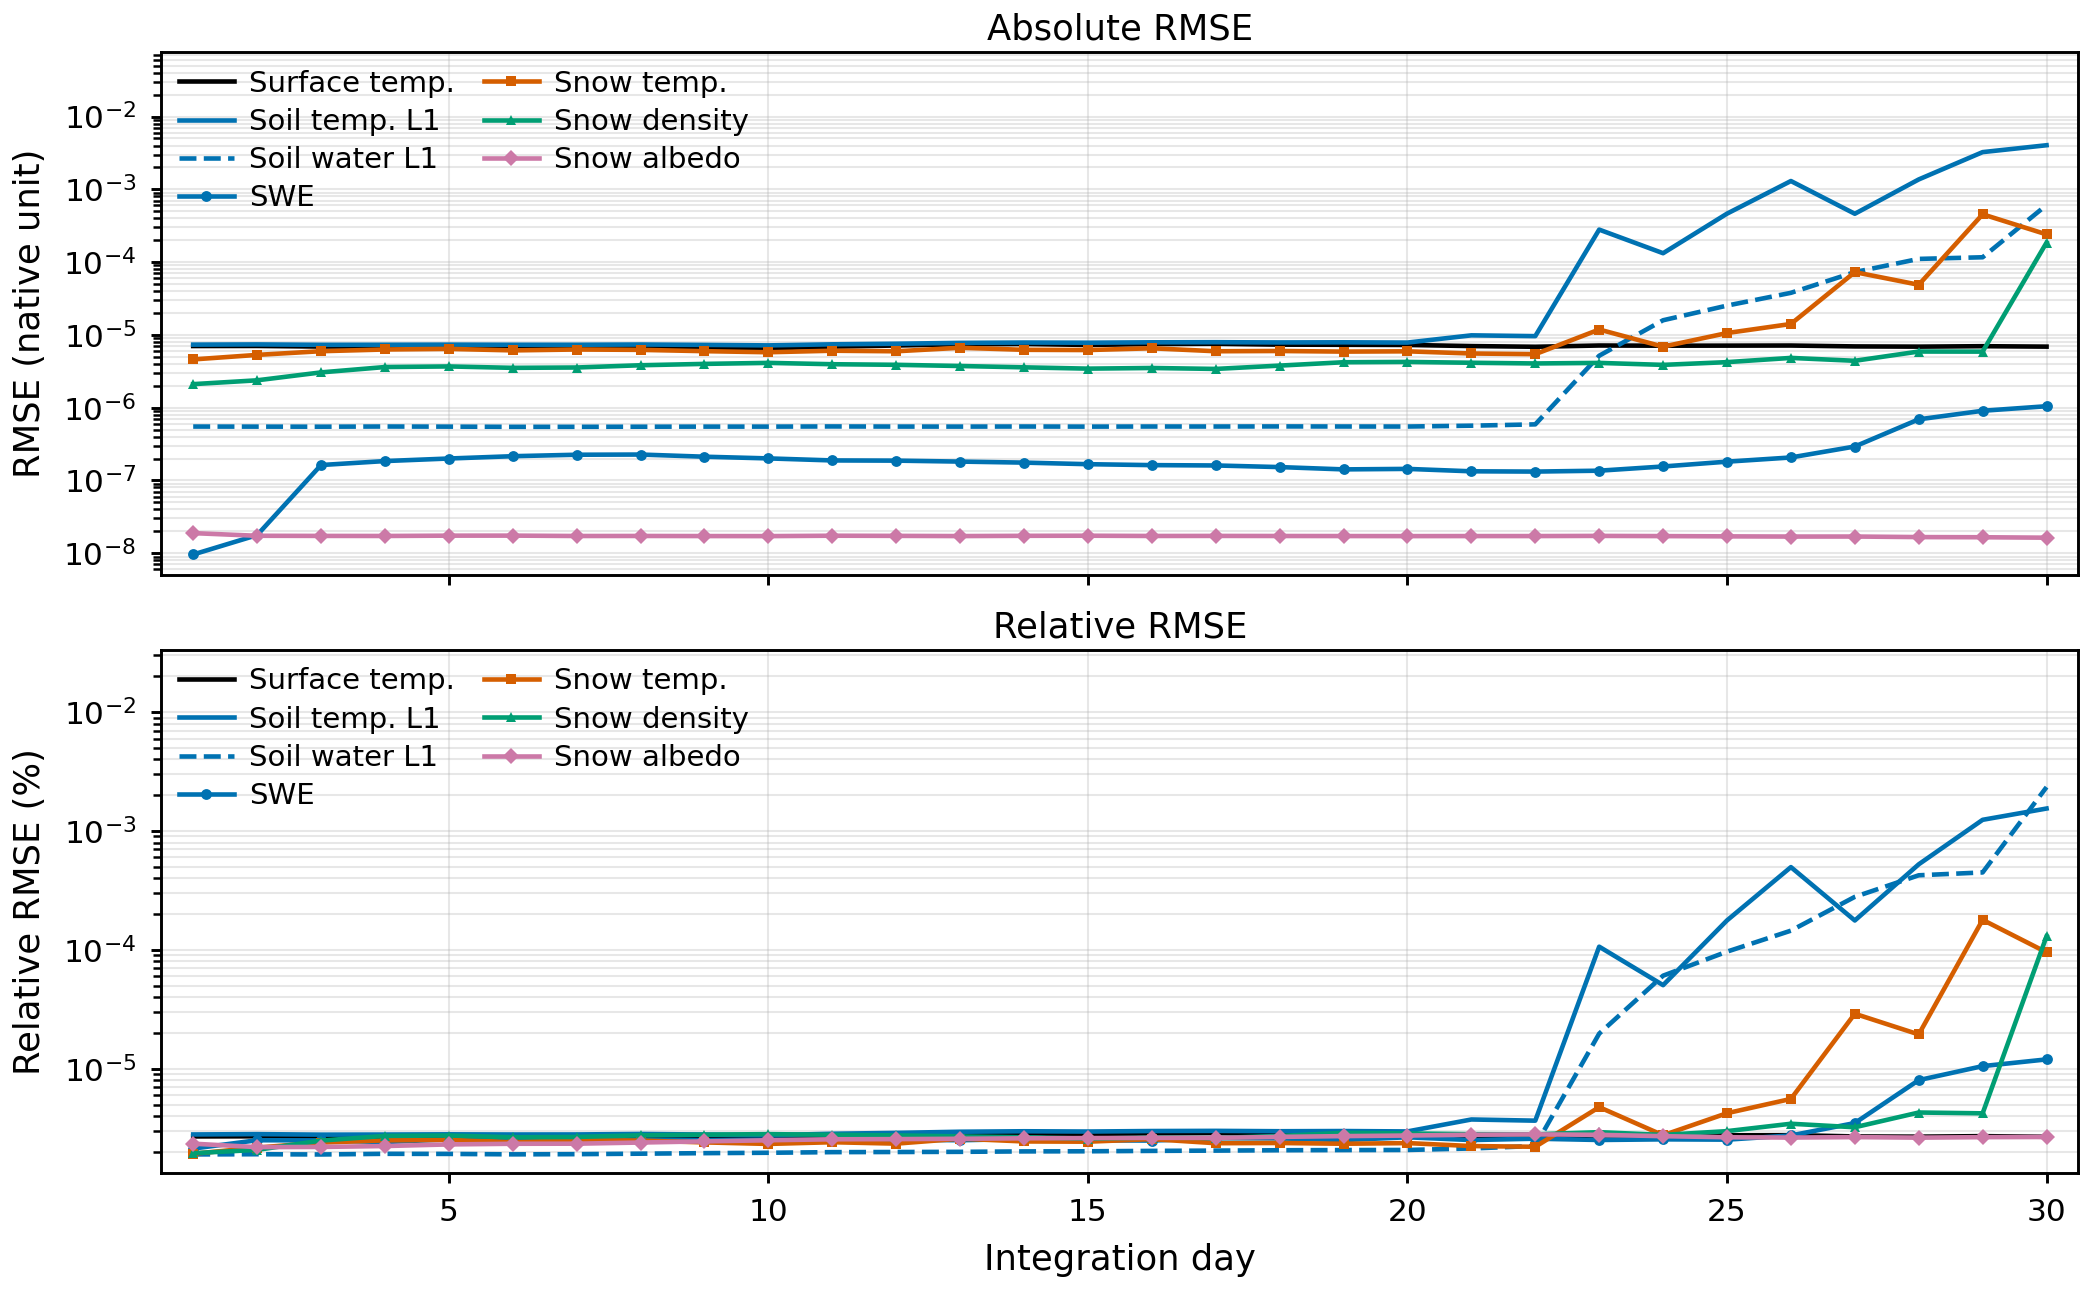
\includegraphics[width=\linewidth]{figures/controlled_30d_20260807/controlled_30d_error_growth.png}
\caption{Error evolution during the continuous 30-day controlled full-domain
boundary-driven integration. Every PyTorch step uses Fortran-captured roughness, surface-layer
exchange, and radiation boundaries. Absolute and relative RMSE use the masks
described in
Table~\ref{tab:controlled-30d}.}
\label{fig:controlled-error-growth}
\end{figure}

\begin{figure}[t]
\centering
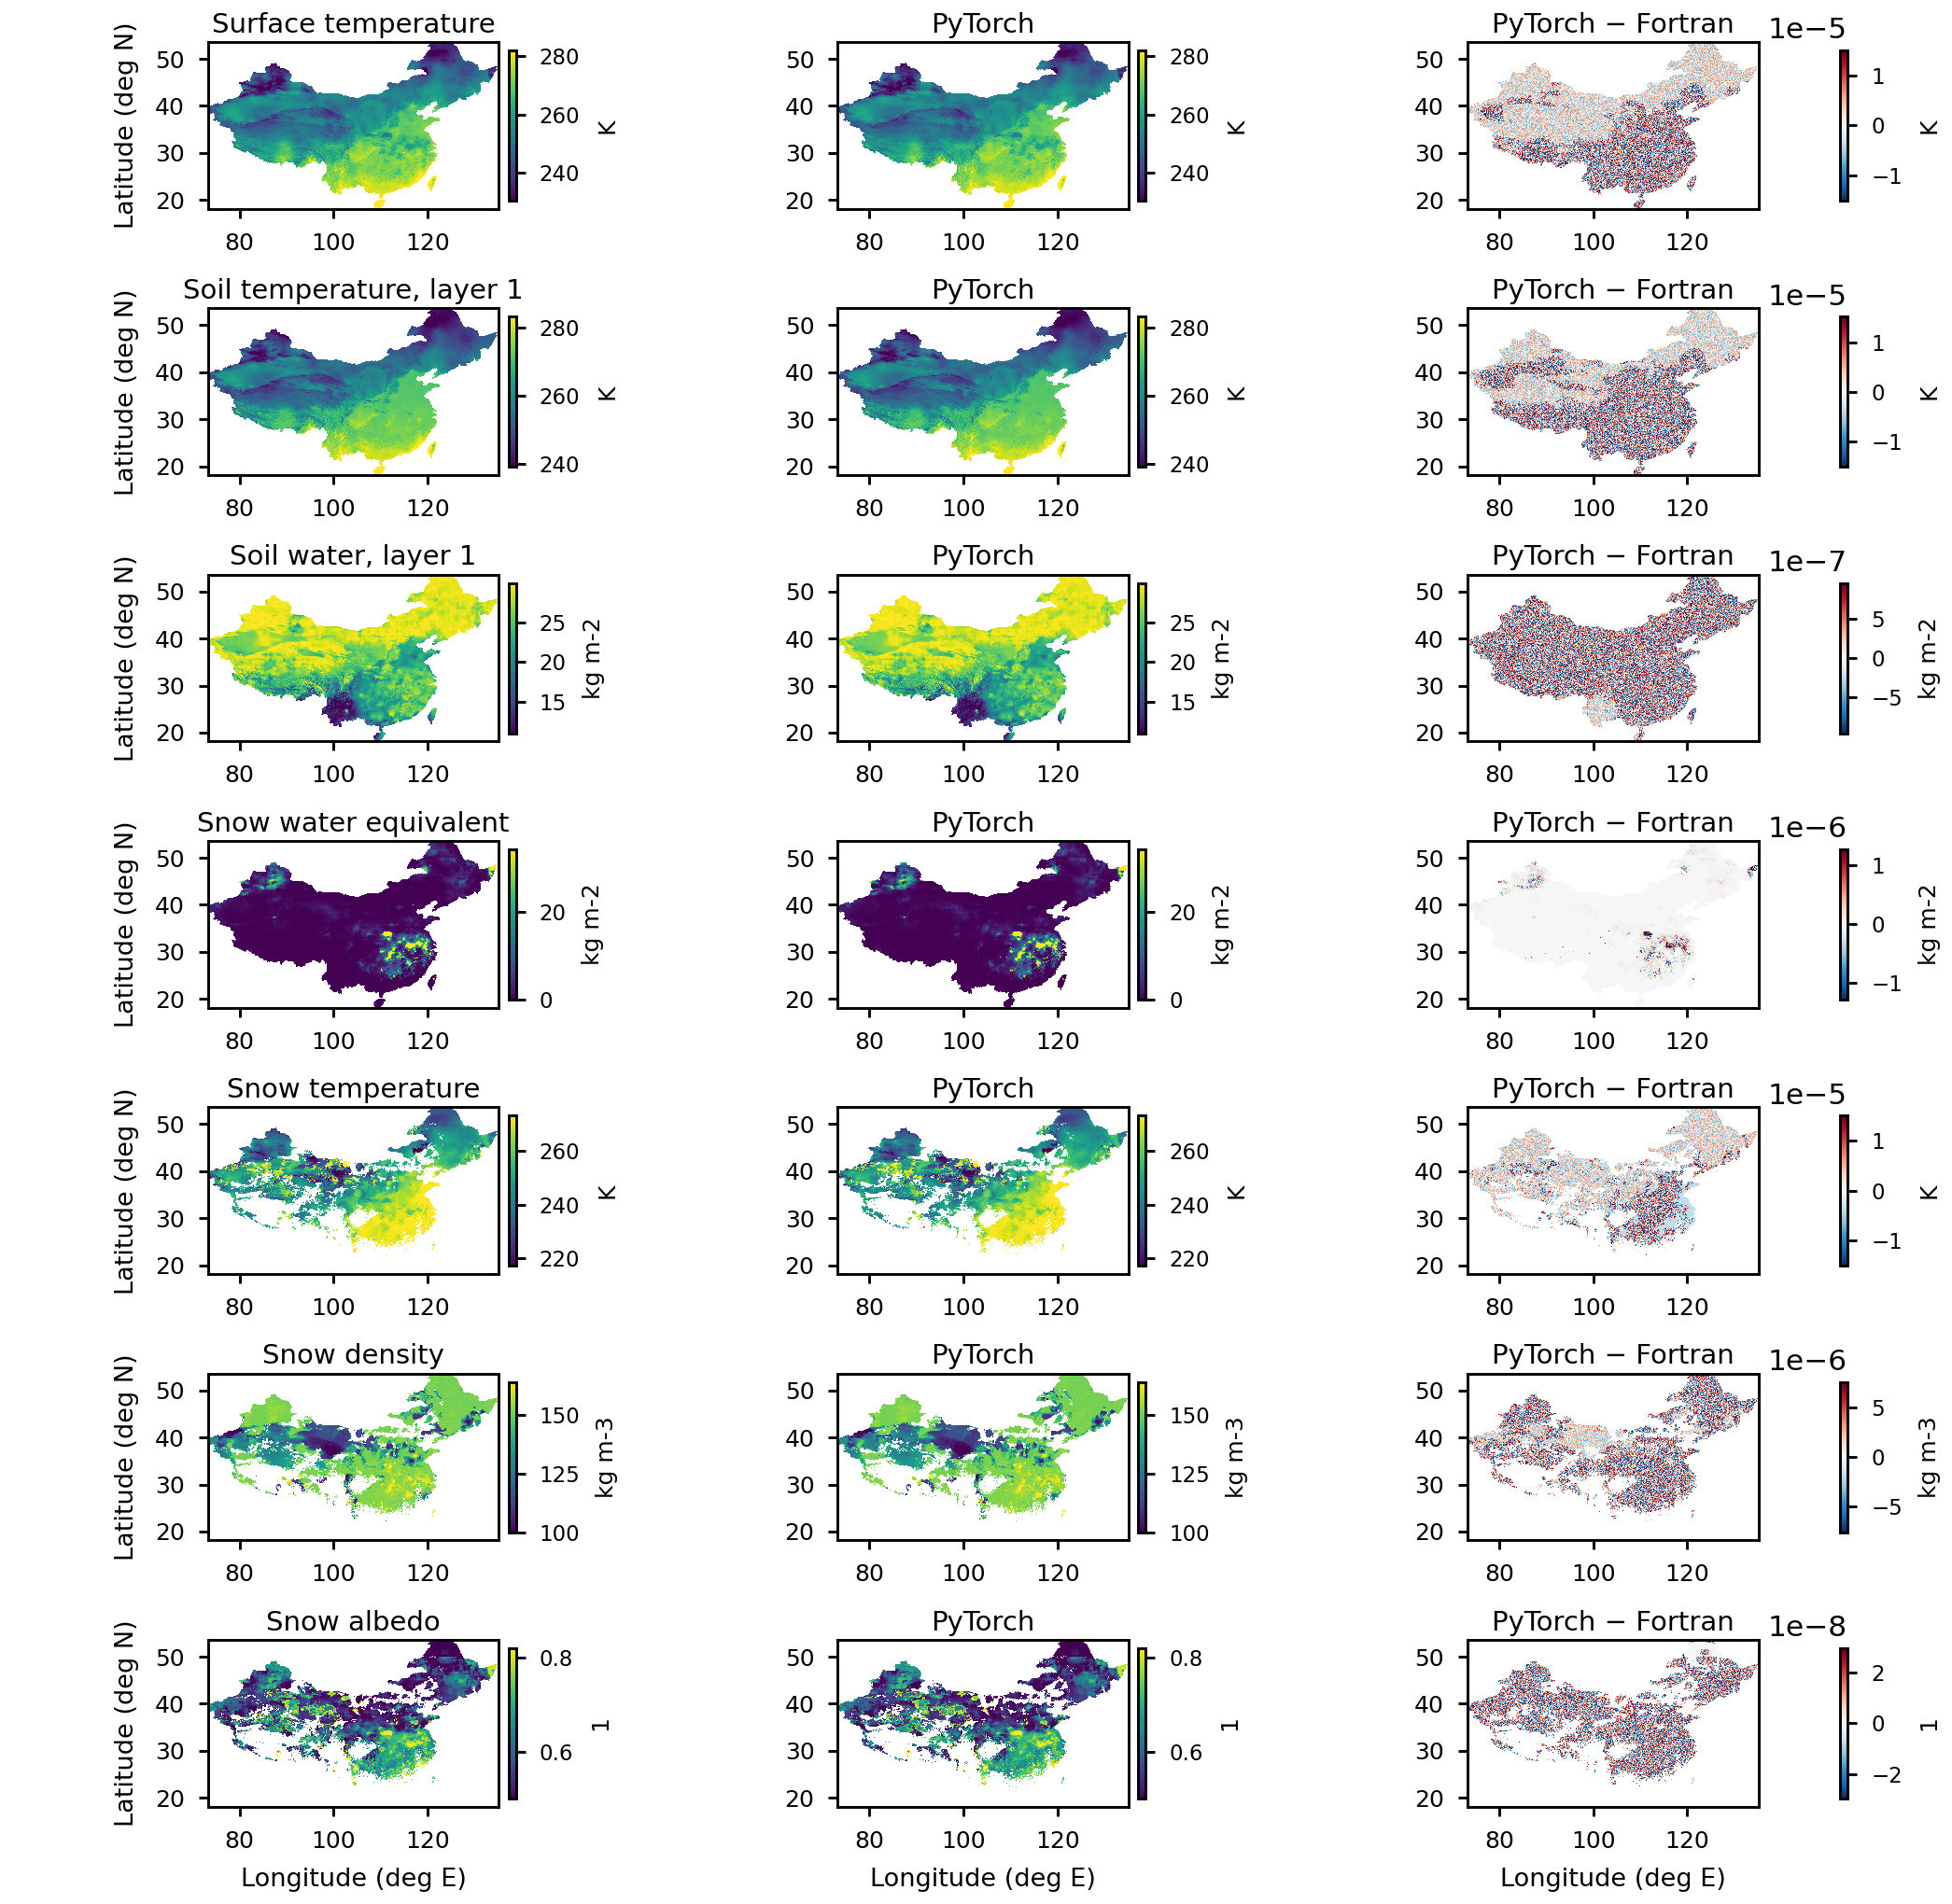
\includegraphics[width=\linewidth,height=0.84\textheight,keepaspectratio]{figures/controlled_30d_20260807/controlled_30d_terminal_maps.png}
\caption{Day-30 controlled full-domain comparison on the original CMFD grid.
Each row is one field; columns show the Fortran state, PyTorch state, and
signed PyTorch minus Fortran difference. Snow diagnostic maps use the
resolved-snow mask. Error colour limits are robust percentile limits.}
\label{fig:controlled-maps}
\end{figure}

The 30-day and one-year experiments serve different verification purposes.
The former is a boundary-controlled test of the translated sequence:
identical Fortran-generated roughness, surface-layer exchange, and radiative
boundary fields remove atmospheric-closure differences and
allow the translated SURF process sequence to be examined directly. The
latter
is a system-level offline test: each implementation constructs its own
boundary state from the common forcing and is therefore sensitive to both the
SURF translation and the standalone atmospheric-surface closure. The two
experiments are consequently complementary rather than repeated integrations.

\subsection{One-year autonomous offline integration}
\label{sec:annual-autonomous-equivalence}

The controlled experiment verifies the SURF process sequence given the
atmospheric boundary. The more demanding autonomous experiment verifies the
complete offline pathway in which each implementation constructs its own
roughness and surface-layer exchange state. Both models start from the same
common spun-up initial state described above and use the
same 2018 CMFD forcing, 1800~s time step, three-hour forcing interpolation,
and precipitation/radiation alignment. The 97,709-column integration runs
for 17,520 continuous steps (365~d), with states archived every 480 steps
(10~d) and at the terminal step. No non-finite values occur in any saved
PyTorch prognostic field.

Fortran writes state snapshots every 480 steps through day~360, and a separate
Fortran integration with the same initial state, forcing, and numerical settings
writes the day-365 terminal state, differing only in output frequency. PyTorch stores the same 10-day sequence plus the exact
terminal step. Thus Fig.~\ref{fig:annual-error-growth} describes one
continuous year-long integration sampled for diagnosis, not a set of 10-day
forecasts.

As a reference-side reproducibility check, the archived one-year Fortran
experiment was repeated on the same machine from the independently
regenerated forcing file and an identical configuration: all 24 output fields
of the repeat integration, including every soil, snow, and tile state,
are bitwise identical to the archive. The Fortran reference trajectory used
in the comparisons below is therefore deterministic and exactly
reproducible, so any Fortran--PyTorch difference is attributable to the
translation and not to run-to-run variability of the reference.

The PyTorch side is checked with the same rigour. Repeated integrations from
a given restart are bitwise identical, and re-integrating the first 30~d of the
multi-year integration of Sect.~\ref{sec:multiyear} through the
same code path as the experiments reproduces the archived records bit for
bit on both accelerator architectures used in this study (NVIDIA
RTX~A6000 and A100). Reproducibility does, however, extend only as far as the pinned
software stack. A decade integration launched under a different PyTorch
build ($2.6.0$+cu124 instead of the pinned $2.11.0$+cu130; all arithmetic
remains float64) departs from the pinned-build trajectory at last-bit
rounding level within the first days (day-10 snow-water maximum difference
$7.2\times10^{-8}$~kg~m$^{-2}$). The offline snow--soil feedback then
amplifies these last-bit seeds to about $1.1\times10^{-3}$~kg~m$^{-2}$ rms
snow water and locally up to 2.8~K skin temperature by the end of the first
year, with unchanged physics and identical inputs. Every experiment
reported in this paper therefore runs in a single pinned environment
(Python 3.10, PyTorch 2.11.0+cu130), and the manifest of each archived
experiment records the interpreter, the PyTorch and CUDA builds, and
SHA-256 hashes of every source file, in addition to the input and output
digests.

\begin{table}[t]
\caption{Day-365 Fortran--PyTorch comparison for the autonomous offline
CMFD integration. Relative RMSE is normalized by the root-mean-square
Fortran field over the stated mask. ``All'' contains 97,709 columns; the
resolved-snow mask contains 82,112 columns at day~365.}
\label{tab:annual-autonomous}
\centering
\small
\begin{tabular}{llrr}
\hline
Quantity (unit) & mask & RMSE & relative RMSE (\%) \\
\hline
Soil temperature, layer 1 (K) & all & $2.83\times10^{-4}$ & $1.07\times10^{-4}$ \\
Soil temperature, layer 2 (K) & all & $2.38\times10^{-4}$ & $8.94\times10^{-5}$ \\
Soil temperature, layer 3 (K) & all & $1.72\times10^{-4}$ & $6.32\times10^{-5}$ \\
Soil temperature, layer 4 (K) & all & $1.22\times10^{-4}$ & $4.34\times10^{-5}$ \\
Soil water, layer 1 (kg m$^{-2}$) & all & $4.19\times10^{-4}$ & $2.43\times10^{-3}$ \\
Soil water, layer 2 (kg m$^{-2}$) & all & $1.36\times10^{-3}$ & $2.54\times10^{-3}$ \\
Soil water, layer 3 (kg m$^{-2}$) & all & $6.22\times10^{-3}$ & $3.24\times10^{-3}$ \\
Soil water, layer 4 (kg m$^{-2}$) & all & $5.55\times10^{-3}$ & $1.03\times10^{-3}$ \\
Snow water equivalent (kg m$^{-2}$) & all & $7.15\times10^{-4}$ & $2.61\times10^{-4}$ \\
Snow temperature (K) & $f_{\rm snow}>10^{-3}$ & $2.30\times10^{-4}$ & $9.08\times10^{-5}$ \\
Snow density (kg m$^{-3}$) & $f_{\rm snow}>10^{-3}$ & $7.22\times10^{-3}$ & $5.02\times10^{-3}$ \\
Snow albedo (-) & $f_{\rm snow}>10^{-3}$ & $3.72\times10^{-6}$ & $6.44\times10^{-4}$ \\
\hline
\end{tabular}
\end{table}

The annual error evolution is shown in Fig.~\ref{fig:annual-error-growth}.
Differences remain small throughout the cold-season spin-up and increase
locally during the spring snow evolution, when round-off-scale differences
can traverse different density, phase, or cover thresholds. They do not
produce a monotonic domain-wide drift: at day~365 the largest relative RMSE
among the prognostic fields is $3.2\times10^{-3}$\% (layer-3 soil water),
the resolved-snow diagnostics reach $5.0\times10^{-3}$\% (snow density),
and all soil-temperature relative RMSE values are
below $1.1\times10^{-4}$\%. The terminal fields are compared on the original
CMFD grid in Figs.~\ref{fig:annual-soil-temperature-maps},
\ref{fig:annual-soil-water-maps}, and~\ref{fig:annual-snow-maps}:
the signed differences remain small everywhere relative to the state
amplitudes, with no coherent spatial structure.

Table~\ref{tab:annual-autonomous} reports the pinned source revision whose
SHA-256 hashes are recorded in the experiment manifest; this is the same
revision as the decadal integration of Sect.~\ref{sec:multiyear}. An
earlier code state of the same implementation, since superseded and not
byte-archived, reached about ten times smaller terminal RMSE
($3.5\times10^{-4}$~K layer-1 soil temperature). Comparing the two
trajectories column by column localizes the effect of the code change:
at day~10, 93\% of the 97,709 columns are bitwise identical (median
absolute difference $6\times10^{-14}$~K) and only 59 columns differ by more
than $10^{-3}$~K (maximum $3.3\times10^{-2}$~K), all of them at states that
sit on discrete phase, snow-cover, or stability thresholds. The residual
Fortran--PyTorch difference of the autonomous configuration is therefore
governed by round-off-seeded selection among discrete physical branches,
not by formula or unit discrepancies, and its amplitude depends on the
exact source revision; the controlled boundary-driven integration of
Sect.~\ref{sec:controlled-equivalence}, which prescribes the atmospheric
boundary, is insensitive to this mechanism.

\subsection{Annual water and energy-budget diagnostics}
\label{sec:annual-budget}

The absence of non-finite values is supplemented by an explicit column water
budget. For each 1800~s step, the diagnostic accumulates total precipitation,
the signed surface moisture flux, surface and subsurface runoff, and changes
in the four-layer soil, snow, and skin-reservoir water stores. The discrete
residual is
\begin{equation}
 \epsilon_W = \Delta S - (P+E-R_s-R_d),
\label{eq:water-residual}
\end{equation}
where evaporation is negative when it removes water from the column. Over the
full domain and year, the mean terms are $P=634.78$, $E=-511.05$,
$R_s=64.16$, $R_d=8.96$, and $\Delta S=50.62$~kg~m$^{-2}$. The terminal
residual has an RMS of $5.90\times10^{-12}$~kg~m$^{-2}$ and a maximum absolute
value of $3.45\times10^{-11}$~kg~m$^{-2}$, corresponding to
$3.76\times10^{-13}\%$ of the mean annual water-throughput scale. This
diagnostic is calculated from the prognostic update and is not fed back into
the integration.

The lower-left panel of Fig.~\ref{fig:annual-budget} reports the associated
surface-energy diagnostic. The two summary measures are
\begin{equation}
\begin{aligned}
 \overline{\epsilon_E} &= -0.123~\mathrm{W\,m^{-2}},\\
 \overline{|\epsilon_E|} &= 3.87~\mathrm{W\,m^{-2}},
\end{aligned}
\label{eq:energy-residual}
\end{equation}
where the first quantity is the signed annual domain mean and the second is
the mean absolute instantaneous residual. The latter is retained as a
diagnostic measure because the
implicit surface-energy solve, tile shortwave transmission, longwave
reweighting, and snow-under-vegetation correction are evaluated in separate
discrete stages. It is therefore not interpreted as an additional prognostic
source or sink.

\begin{figure}[t]
\centering

\includegraphics[width=\linewidth]{figures/annual_repro_gpunative/annual_autonomous_error_growth.png}
\caption{Absolute and relative Fortran--PyTorch error evolution during the
continuous one-year autonomous offline integration. The saved 10-day states
and day-365 terminal state are samples from the same integration. Three
representative fields are shown: snow water equivalent, layer-1 soil
temperature, and snow temperature. The fields not plotted stay within the
following ranges over the year: layers 2--4 of soil temperature,
$6.4\times10^{-6}$--$4.8\times10^{-4}$\,\%; layers 1 and 4 of soil water,
$2.4\times10^{-6}$--$1.3\times10^{-2}$\,\%; snow density and albedo on the
resolved-snow mask, $7.7\times10^{-6}$--$1.9\times10^{-2}$\,\% and
$2.3\times10^{-6}$--$6.4\times10^{-3}$\,\% respectively. Snow temperature is
masked at a snow-cover fraction above $10^{-3}$.}
\label{fig:annual-error-growth}
\end{figure}

\begin{figure}[t]
\centering

\includegraphics[width=\linewidth]{figures/annual_repro_gpunative/annual_autonomous_terminal_soil_temperature_maps.png}
\caption{Day-365 full-domain comparison for all four soil-temperature layers.
Each row is one layer; columns show the Fortran state, PyTorch state, and
signed PyTorch minus Fortran difference. Difference colour limits use the
99.5th percentile of the absolute error.}
\label{fig:annual-soil-temperature-maps}
\end{figure}

\begin{figure}[t]
\centering

\includegraphics[width=\linewidth]{figures/annual_repro_gpunative/annual_autonomous_terminal_soil_water_maps.png}
\caption{Day-365 full-domain comparison for all four soil-water layers.
Each row is one layer; columns show the Fortran state, PyTorch state, and
signed PyTorch minus Fortran difference. Difference colour limits use the
99.5th percentile of the absolute error.}
\label{fig:annual-soil-water-maps}
\end{figure}

\begin{figure}[t]
\centering

\includegraphics[width=\linewidth,height=0.95\textheight,keepaspectratio]{figures/annual_repro_gpunative/annual_autonomous_terminal_snow_maps.png}
\caption{Day-365 full-domain comparison for snow water equivalent, snow
temperature, snow density, and snow albedo. Each row is one field; columns
show the Fortran state, PyTorch state, and signed PyTorch minus Fortran
difference. The snow diagnostic fields use the $f_{\rm snow}>10^{-3}$ mask.
Difference colour limits are robust percentile limits.}
\label{fig:annual-snow-maps}
\end{figure}

\begin{figure}[t]
\centering
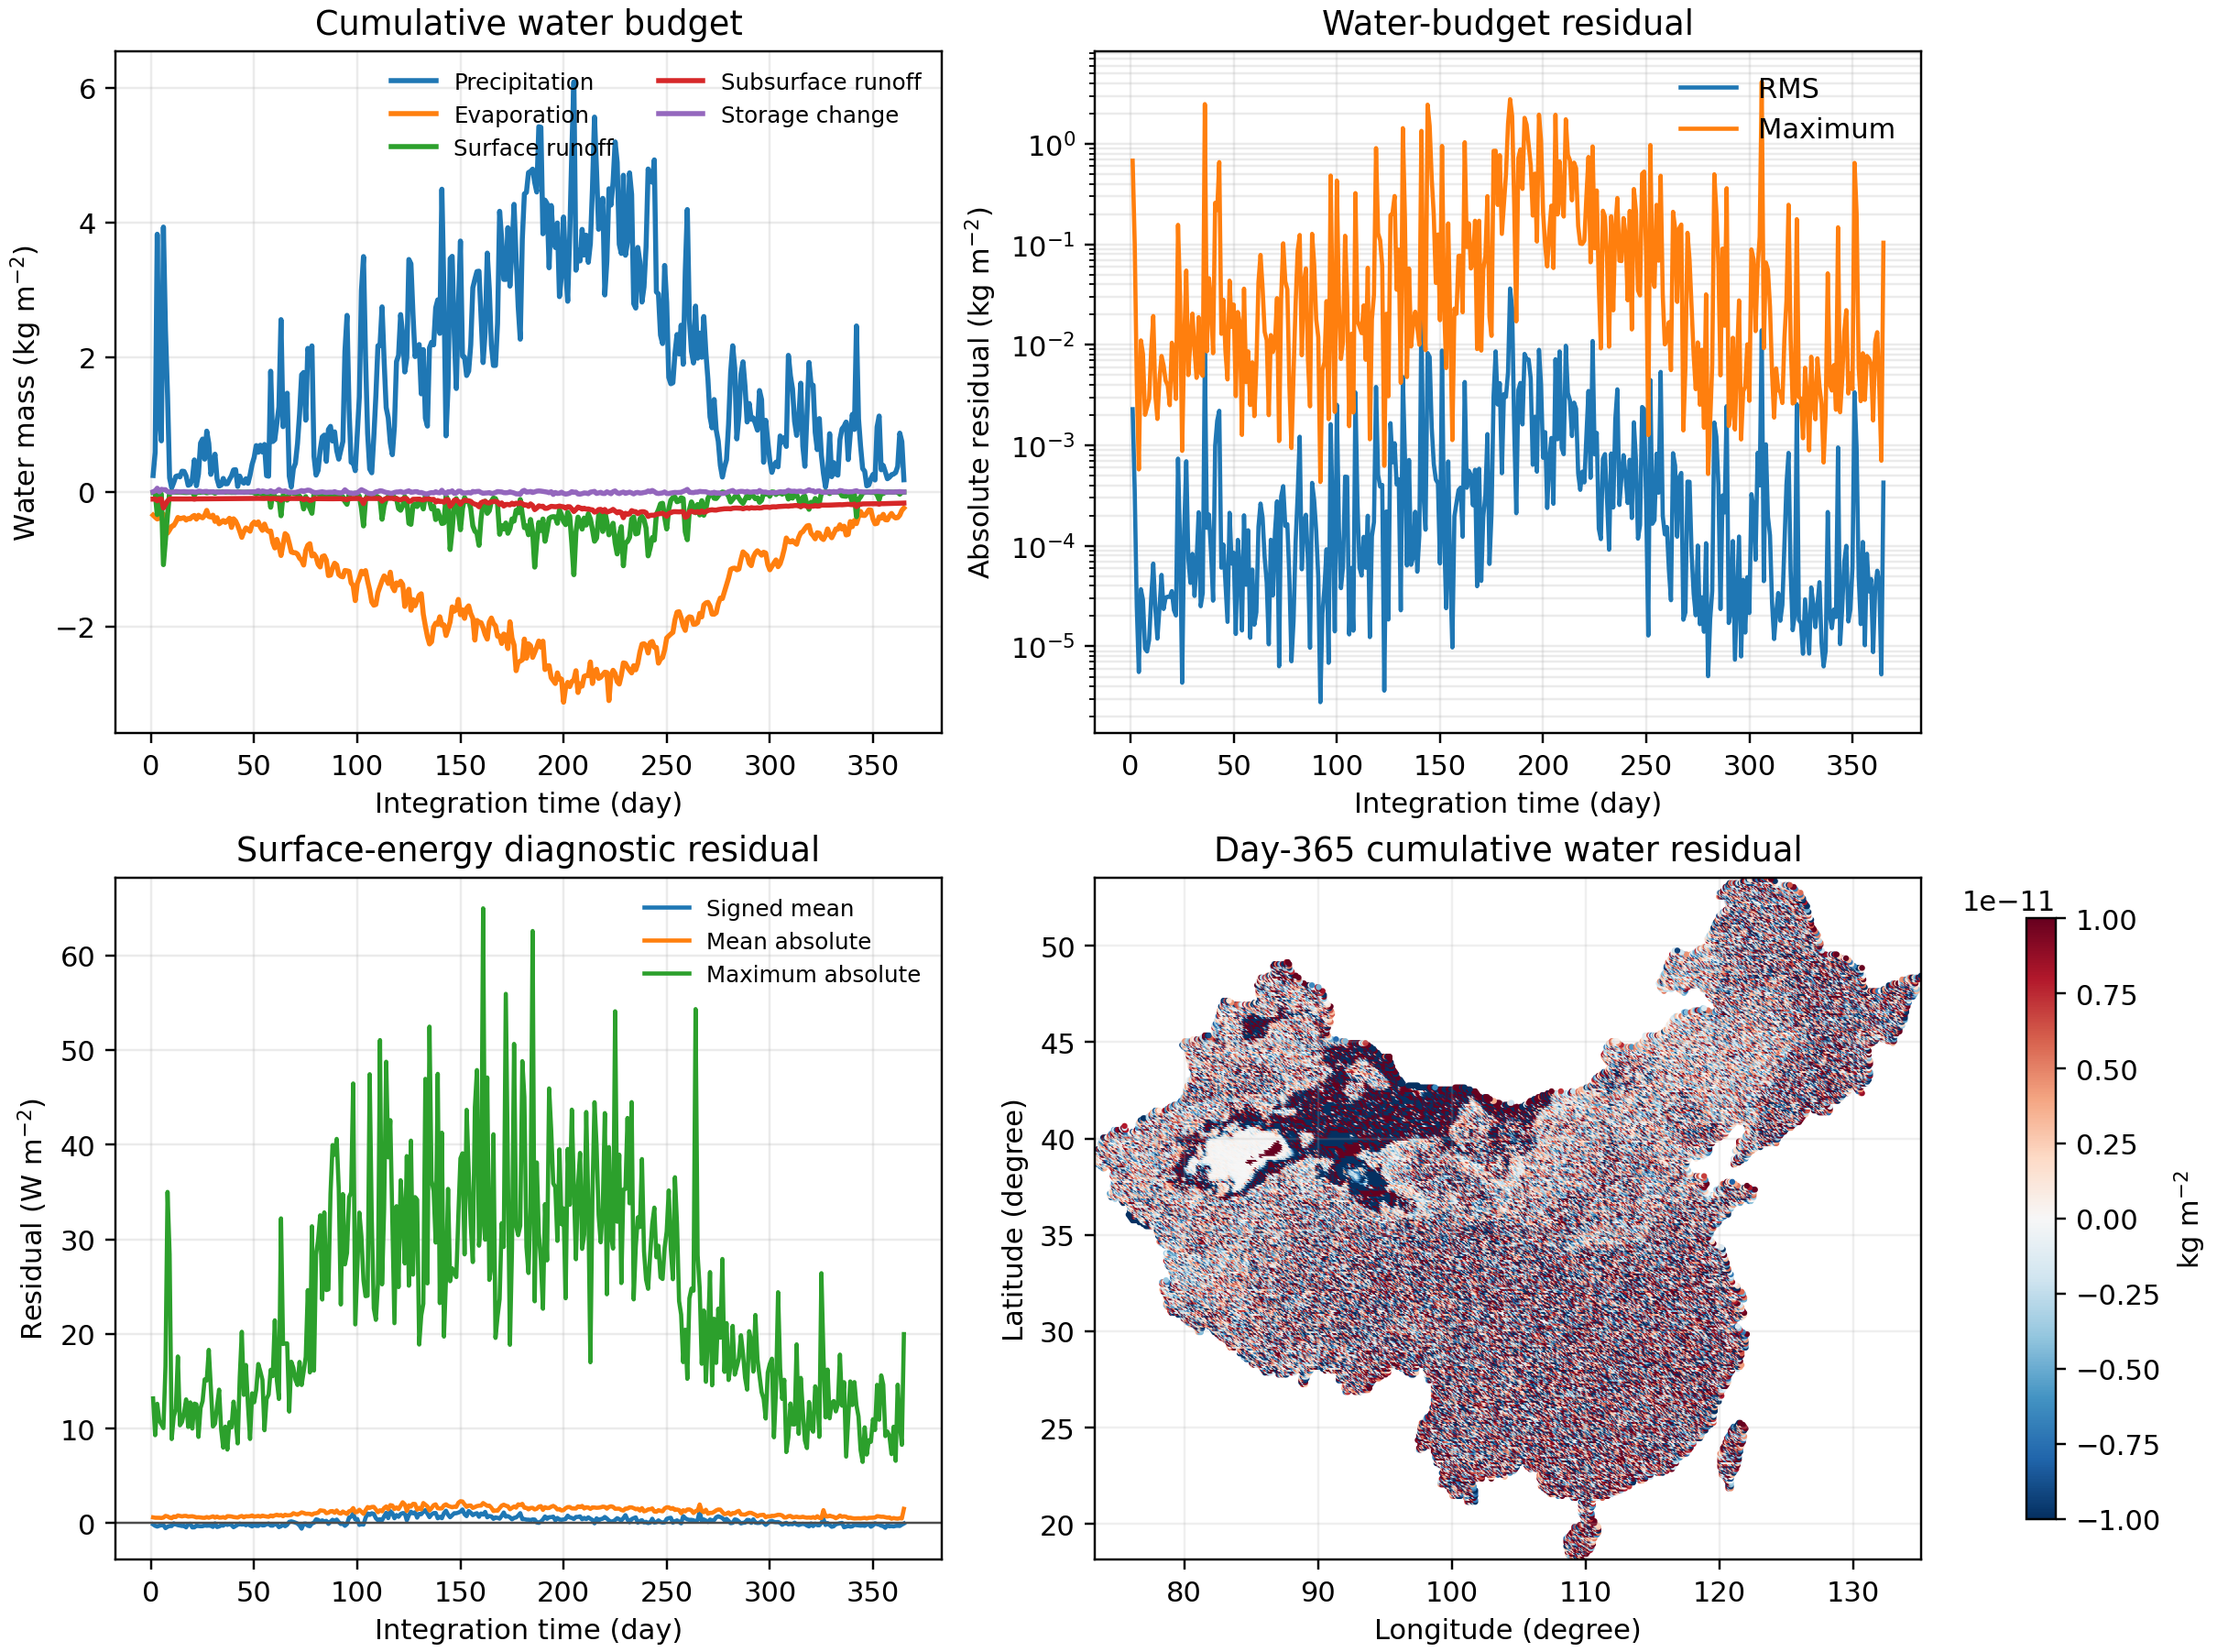
\includegraphics[width=\linewidth]{figures/annual_water_energy_budget.png}
\caption{Annual water and energy-budget diagnostics for the continuous
97,709-column Torch integration. Upper left: domain-mean cumulative water
terms, with outward fluxes plotted negative. Upper right: cumulative water
residual. Lower left: signed and absolute surface-energy diagnostic residual.
Lower right: day-365 cumulative water residual on the original CMFD
longitude--latitude locations.}
\label{fig:annual-budget}
\end{figure}
